\documentclass{beamer}

 \usepackage{beamerthemesplit}
% \usepackage[danish]{babel}
\usepackage[utf8]{inputenc}
% \usepackage{graphics}
\usepackage{graphicx}
% \usepackage{epsfig}
\usepackage{subfigure}
 \usepackage{url}
 \usepackage{amsmath}
\usepackage{amssymb}
 \usepackage{algorithmic}

% \DeclareGraphicsExtensions{.pdf,.png,.jpg,.eps}
\graphicspath{{./}}

\definecolor{kugreen}{RGB}{50,93,61}
\definecolor{kugreenlys}{RGB}{132,158,139}
\definecolor{kugreenlyslys}{RGB}{173,190,177}
\definecolor{kugreenlyslyslys}{RGB}{214,223,216}

\setbeamercovered{transparent} \mode<presentation> {
  \usetheme{Copenhagen} \usecolortheme[named=kugreen]{structure}
  \useinnertheme{circles} \usefonttheme[onlymath]{serif}
  \setbeamercovered{transparent}
  \setbeamertemplate{blocks}[rounded][shadow=true] }
% \setbeamertemplate{background}{\includegraphics[width=1\textwidth]{natfak_baggrund.pdf}}
% \logo{\includegraphics[width=1cm]{billeder/logo}}

\title{High Performance Query Execution in Analytical Databases over a
  Scalable Heterogeneous Distributed Environment with Fault Tolerance}
 % \subtitle{Presentation for the Course: High Dimensional Data Management}
\author{Abu Zaher Md. Faridee 
% (0411052040) 
\\  Samir Hasan
  % (0411052067)
\\ Wasik Mursalin Rushafi 
% (0411052065)
}
\institute{Department of Computer Science\\Bangladesh University of
  Engineering and Technology} \date{\today{}}
% Presentation for the Course: High Dimensional Data Management

\begin{document}

\frame{ \titlepage
  % \vspace{-0.5cm}
  % \begin{center}
  %   %   \includegraphics[height=0.25\textheight]{billeder/polygons}
  % \end{center}
}

\frame{ \frametitle{Overview}
  \tableofcontents[pausesection]
}

% \begin{block}{Kryptering med kaotiske kredsløb}
%   \begin{columns}
%     \column{.3\textwidth} \hspace{0.5cm}
%       %     \includegraphics[width=0.7\textwidth]{billeder/circuit}
%     \column{.7\textwidth} \textit{Mogens Høgh Jensen}, NBI
%   \end{columns}
% \end{block}

\section{Introduction}
\label{sec:introduction}

% \subsection{The Longest Path Problem}
% \label{sec:problem-definition}

\subsection*{Problem Definition}
\label{sec:problem-definition}

\begin{frame}
  \frametitle{Problem Definition}
  % \begin{block}{}
      Given explosive amounts of data, design an analytical database
  system that features performance, scalability, fault tolerance and
  a flexible query interface

  % \end{block}
\end{frame}

% \frame{

%   \frametitle{The Longest Path Problem}

%   \begin{block}{Definition}

%     Given an undirected graph $G = (V, E)$, where $V$ is the set of
%     $n$ vertices and $E$ is the set of $m$ edges, for all $u, v \in
%     V$, find the highest cost path from $u$ to $v$, visiting a vertex
%     only once
%   \end{block}

%   \begin{itemize}
%   \item For \emph{Weighted Graphs}, the \emph{Longest Path} is the
%     path that has the highest sum of weights of it's edges
%   \item For \emph{Unweighted Graphs}, the \emph{Longest Path} is the
%     path that contains the most number of edges
%   \item Covering all the vertices is not mandatory
%   \end{itemize}

% }


% \frame{
%   \frametitle{Example}
%   The bold edges denote the longest path for this graph, total cost is
%   45
%   \begin{center}
%     \includegraphics[width=0.7\textwidth]{lpath-best-sol}
%   \end{center}
% }

% \frame{
%   \frametitle{NP-Completeness}
%   \begin{block}{Reduction from \emph{Hamiltonian Path} Problem}
%     \begin{itemize}
%     \item Given an instance $G' = (V' ,E')$ for \emph{Hamiltonian
%         Path}, count the number $|V'|$ of nodes in $G'$ and output the
%       instance $G = G',K = |V '|$ for \emph{Longest Path}.
%     \item $G'$ has a simple path of length $|V'|$ if and only if
%       $|G'|$ has a Hamiltonian path.
%     \end{itemize}
%   \end{block}
%   The problem is NP-Complete even if there is no \emph{Hamiltonian
%     Path}, as we are trying to visit as much vertices as possible }


\subsection{Motivation}
\label{sec:motivation}

\begin{frame}
  \frametitle{Major Trends}
  \begin{itemize}
  \item Data Explosion
    \begin{itemize}
    \item Automation of business processes, proliferation of digital
      devices
    \item eBay has a 6.5 petabyte warehouse.
    \end{itemize}
   \item Deep Analysis over Raw Data
     \begin{itemize}
     \item Inefficient to push data from database into specialized analysis
       engines $\rightarrow$ process data in the database
     \item Best price/performance $\rightarrow$ data partitioned across 100-1000s
       of cheap, commodity, shared-nothing machines.
     \item Clouds of processing nodes on demand, pay for what you use
    \end{itemize}
  \end{itemize}
  \begin{block}{Bottom Line}
    Processing massive structured data on 1000s of shared-nothing
    nodes
  \end{block}
\end{frame}

\begin{frame}
  \frametitle{Analytical Data Processing}
  \begin{itemize}
  \item Online Analytical Processing (OLAP) is an approach to swiftly
    answer online multi-dimensional analytical (MDA)
    queries. %[Ref. http://en.wikipedia.org/wiki/Online_analytical_processing
  % \item It is a read-only system that stores historical data on business
  %   metrics.
  \item Analytical Data Processing are done through Analytical Databases
    which are often distributed systems among tens of nodes that
    incorporate MPP (Massively Parallel Processing System)
  \item The Analytical database market is growing steeply.
  \item As of 2006 it consists of \$3.98 billion of the \$14.6 billion
    database software market (27\%). Since then it is growing at a rate of 10.3\% annually.
  \end{itemize}
\end{frame}

\subsection{Main Challenges}
\begin{frame}
  \frametitle{Desired properties of a Data Analysis System in the
    Petabyte Scale}
  \begin{itemize}
  \item {\bfseries{Performance}}: The system should be able run
    optimized data analysis algorithms within the available hardware
    resources.
  \item {\bfseries{Fault Tolerance}}: For transactional workloads it should recover
    from a failure without losing any data / updates from recently
    committed transactions.
  \item {\bfseries{Performance in Heterogeneous System}}: The system should perform
    well with the addition more nodes which are varies in performance.
  \item {\bfseries{Flexible Query Interface}}: Users should be able to querying the database over the network just like normal databases.
  \end{itemize}
\end{frame}

% \frame{
%   \frametitle{Applications}
%   \begin{itemize}
%   \item Appears as a subproblem in path planning, networking and in
%     many other industrial and logistic applications
%   \item Portugal and Rocha [cite needed] used \emph{Longest Path} to
%     patrol a graph with multiple robots when there is no
%     \emph{Eulerian} and \emph{Hamiltonian Path}
%   \end{itemize}
% }

% \subsection{Research Challenges}

% \frame{
%   \frametitle{Previous Works }

%   \begin{itemize}
%   \item Karger [cite needed] first proposed a polynomial time
%     approximation algorithm for weighted undirected graphs, but with
%     limited performance
%   \item Portugal and Rocha [cite needed] used a \emph{Genetic
%       Algorithm} based approach in 2010
%   \end{itemize}
% }


\section{State of the Art}
\label{sec:state-of-the-art}

% \subsection{Some Background Knowledge}
\begin{frame}
  \frametitle{Shared Nothing Architecture: The popular choice for
    Deploying Distributed Databases}
  \begin{itemize}
  \item A collection of independent (possibly virtual machines with local disk and local main memory) computer systems connected together a high speed network.
  \item This type of systems are widely believed to scale the best.
  \item Data analysis workloads (e.g. large scan operations, multidimensional aggregations, star schema joins) are fairly easy to parallelize across nodes  in a shared nothing network.
  \end{itemize}
\end{frame}

\subsection{Available Approaches}

\begin{frame}
  \frametitle{Parallel DBMS}
  \begin{itemize}
  \item Analytical DBMS System deployed on a shared nothing
    architecture.
  \item Winner in the performance category.
  \item Modern systems usually have great Query Interface which do no require highly trained DBAs
  \item Do not run well in Heterogeneous environment. Very few systems
    can do well in a hundred node system. And there are no reported
    thousand node Parallel DBA.
  \item Fault Tolerance level is low. Usually a query has to be restarted if it fails due to some node failure. General assumption is node failures are rare events.
  \end{itemize}
\end{frame}

\begin{frame}
  \frametitle{Map Reduce}
  \begin{itemize}
  \item Process data in a shared nothing architecture in three basic
    steps: Map, Repartition and Reduce.
  \item Plans query execution on runtime which allows Map Reduce to be
    fault tolerant.
  \item Lack of a pre-planned query execution policy results in lesser
    performance.
  \item Perform well in heterogeneous environment by reassigning tasks
    on slower nodes to faster nodes that has completed it’s job.
  \item Flexible Query Interfaces can be incorporated via Query Translators like Apache Hive.
  \end{itemize}
\end{frame}

% \frame{

%   \frametitle{Ant Colony Optimization}
%   \begin{itemize}
%   \item A nature inspired algorithm based on the foraging behavior of
%     ants
%     % \item It's a constructive metaheuristic
%   \item Has been successfully applied to solve several NP-hard
%     combinatorial optimization problems [cite needed], such as
%     traveling salesman problem [cite needed], vehicle routing problem
%     [cite needed], and quadratic assignment problem [cite needed]
%   \end{itemize}

% }

% \frame{
%   \frametitle{The Basics of ACO}
%   \begin{itemize}
%   \item Model the given problem as a searching problem in a graph
%   \item Use artificial ants to construct the best path
%   \item Each ant puts a `trail' on it's discovered solution called
%     `\emph{pheromone}'
%   \item Each ant uses this \emph{`pheromone'} information to gradually
%     construct a better solution
%   \item This \emph{`pheromone'} is the globally shared memory of the
%     ants and the most powerful feature of ACO
%   \end{itemize}
% }

% \frame{
%   \frametitle{The Basic Equations of ACO}
%   \begin{block}{The probabilistic Formula}
%     $p_{k}(r, s) = \left\{
%       \begin{array}{rcl}
%         \frac{\tau(r, s) * \eta(r, s)^{\beta}}{\sum_{u \in M_k}{\tau(r,
%             s) * \eta(r, s)^{\beta}}} & $ if $ s \in M_k\\
%         0 & $ otherwise $
%       \end{array}
%     \right.$
%   \end{block}
% }

\section{HadoopDB:  An Architectural Hybrid of MapReduce and DBMS}

\begin{frame}
  \frametitle{Hadoop Basics}
      \begin{center}
      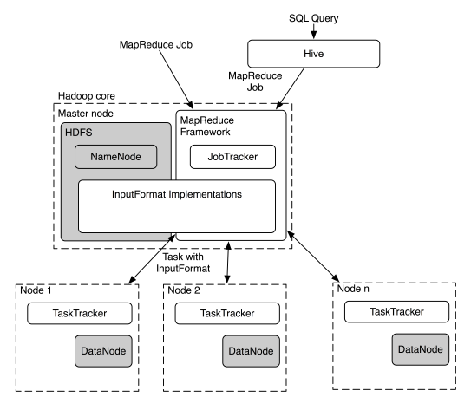
\includegraphics[width=0.7\textwidth]{Hadoop_Basics}
    \end{center}
\end{frame}

\subsection{HadoopDB's Components}
\begin{frame}
  \frametitle{HadoopDB's Components}
  \begin{itemize}
  \item Database Connector
  \item Catalog
  \item Data Loader
  \item SQL to MapReduce to SQL (SMS) Planner
  \end{itemize}
\end{frame}


\begin{frame}
  \frametitle{HadoopDB's  Architecture}
      \begin{center}
      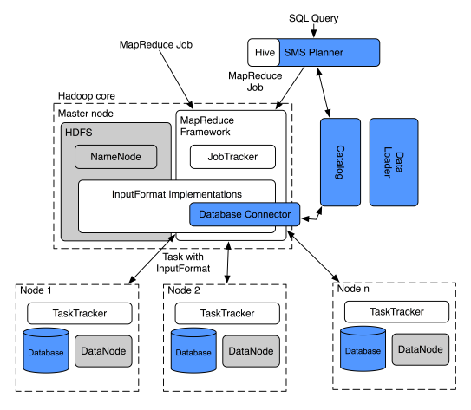
\includegraphics[width=0.7\textwidth]{Architecture}
    \end{center}
\end{frame}

\begin{frame}
  \frametitle{Database Connector}
  \begin{itemize}
  \item Interface between independent database systems residing on nodes in the cluster and TaskTrackers.
  \item Extends Hadoop’s InputFormat class and is part of the Input- Format Implementations library
  \item Connects to the database, executes the SQL query and returns
    results as key-value pairs
    \item By extending Hadoop’s InputFormat, seamless integration with
      Hadoop’s MapReduce Framework is ensured
  \end{itemize}
\end{frame}


\begin{frame}
  \frametitle{Catalog}
  \emph Responsible for maintaining metainformation about
  the databases e.g.
  \begin{itemize}
  \item Connection parameters such as database location, driver class and credentials
  \item Metadata such as data sets contained in the cluster, replica locations, and data partitioning properties
  \end{itemize}
\end{frame}

\begin{frame}
  \frametitle{Data Loader}
  Responsible for
  \begin{itemize}
  \item Globally repartitioning data on a given partition key upon
    loading
  \item Breaking apart single node data into multiple smaller
    partitions or chunks
  \item Bulk-loading the single-node databases with the chunks
  \end{itemize}
Consists of two components
\begin{itemize}
\item The Global Hasher executes a custom- made MapReduce job over
  Hadoop that reads in raw data files stored in HDFS and repartitions
  them into as many parts as the number of nodes in the cluster
\item The Local Hasher copies a partition from HDFS into local file system of each node and secondarily partitions the file into smaller sized chunks based on the maximum chunk size setting
\end{itemize}
\end{frame}

\begin{frame}
  \frametitle{SQL-MR-SQL (SMS): Hive Basics}
  Hive Converts SQL queries into MapReduce jobs over HDFS files
  \begin{itemize}
  \item Derives schema of files from an internal catalog
  \item Parses, plans, optimizes the SQL query into a relational
    operator DAG
  \item Breaks down plan into series of Map / Reduce task with
    interleaving re-partition operators
  \end{itemize}
\end{frame}


\begin{frame}
  \frametitle{SQL-MR-SQL (SMS): Exteding Hive}
  SMS Planner Extends hive in following ways:
  \begin{itemize}
  \item Before any query execution updates the MetaStore with references to database tables
  \item After the physical query plan generation and before the
    execution of the MapReduce jobs, SMS perform two passes over the
    physical plan.
  \item In the first pass, SMS retrieves data fields that are actually
    processed by the plan and determines the partitioning keys used by
    the Reduce Sink (Repartition) operators.
  \item In the second pass, SMS traverse the DAG bottom-up from table scan operators to the output or File Sink operator
  \end{itemize}
\end{frame}

\begin{frame}
  \frametitle{SQL-MR-SQL Review}
  \begin{figure}
    \centering
    \begin{center}
      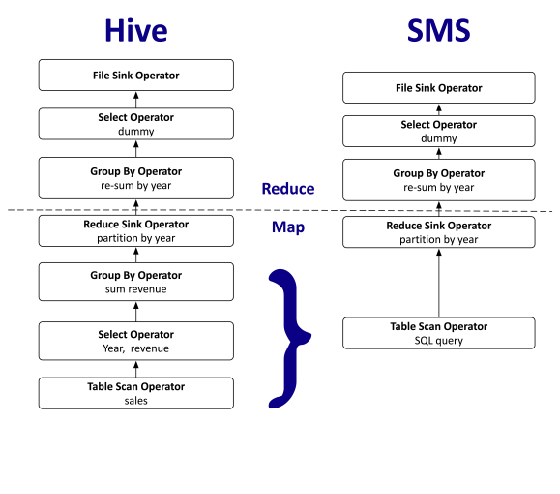
\includegraphics[width=0.5\textwidth]{SQL-MR-SQL}
    \end{center}    
    \caption{   SELECT YEAR(saleDate), SUM(revenue) FROM sales GROUP BY YEAR(saleDate);
    }
  \end{figure}
\end{frame}

\section{Evaluation}
\label{sec:evaluation}

% \subsection{Hypotheses}

\begin{frame}
  \frametitle{Evaluating HadoopDB against Hadoop and Parellel Databases}
  Compare HadoopDB to Hadoop and Parallel databases:
  \begin{itemize}
  \item Performance:
    \begin{itemize}
    \item HadoopDB is expected to approach the performance of
      parallel databases
    \item Load times vs. performance trade-offs
    \end{itemize}
  \item Scalability:
    \begin{itemize}
    \item HadoopDB is expected to scale as well as Hadoop
    \item Fault- and fluctuation- tolerance
    \end{itemize}
  \end{itemize}
\end{frame}

\subsection{Setup}

\begin{frame}
  \frametitle{Experimental Setup}
  \begin{itemize}
  \item Stage
    \begin{itemize}
    \item Amazon EC2 cloud, clusters of 10, 50, 100 machines
    \end{itemize}
  \item Character
    \begin{itemize}
    \item Hadoop
    \item HadoopDB
    \item Vertica
    \item DB-X\footnote{\small{DB-X results reproduced from Pavlo et al. 2009}}%CITE
   \end{itemize}
  \item Plot
    \begin{itemize}
    \item Pavlo et al. SIGMOD benchmark of large-scale analytical
      queries derived from processing web-data
    \item 20+ GB/node
    \end{itemize}
  \end{itemize}
\end{frame}

\subsection{Load}

\begin{frame}
  \frametitle{Load: Grep Data}
  \begin{figure}
    \centering
    \begin{center}
      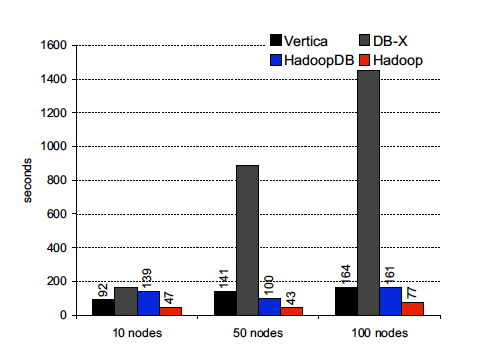
\includegraphics[width=0.6\textwidth]{Load-GrepData}
    \end{center}
    \caption{Grep Data (535MB/node): No pre-processing, data randomly generated}
    \label{fig:load-grep-data}
  \end{figure}
\end{frame}

\begin{frame}
  \frametitle{Load: User Visits Log}
  \begin{figure}
    \centering
    \begin{center}
      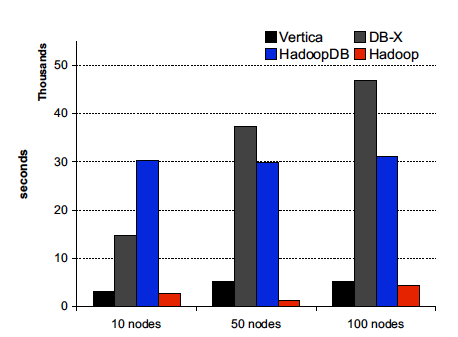
\includegraphics[width=0.6\textwidth]{Load-UserVisitLogs}
    \end{center}
    \caption{User Visits Log (20GB/node): Partitioning, chunking (1GB chunks), sorting and indexing}
    \label{fig:load-user-visit-log}
  \end{figure}
\end{frame}


\subsection{Performance}

\begin{frame}
  \frametitle{Performance: Grep Task}
  \begin{figure}
    \centering
    \begin{center}
      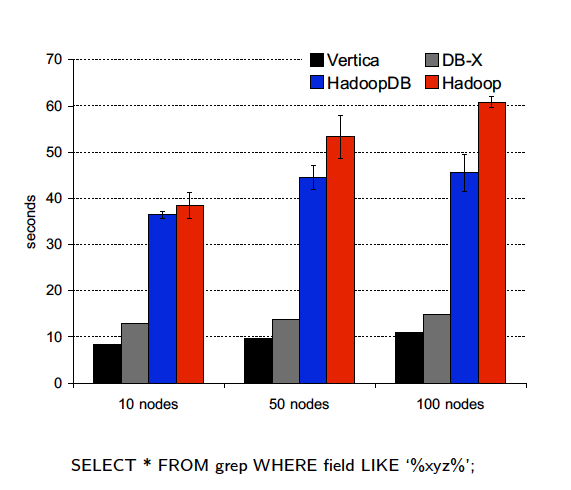
\includegraphics[width=0.6\textwidth]{Performance-Grep-Task}
    \end{center}
    % \caption{SELECT * FROM grep WHERE field LIKE ‘\%xyz\%’;}
 \end{figure}
 % \begin{itemize}
 % \item Full table scan, highly selective filter
 % \item Random data, no room for indexing
 % \item Hadoop overhead outweighs query processing time in single-node databases
 % \end{itemize}
\end{frame}

\begin{frame}
  \frametitle{Performance: Join Task}
    \begin{figure}
    \centering
    \begin{center}
      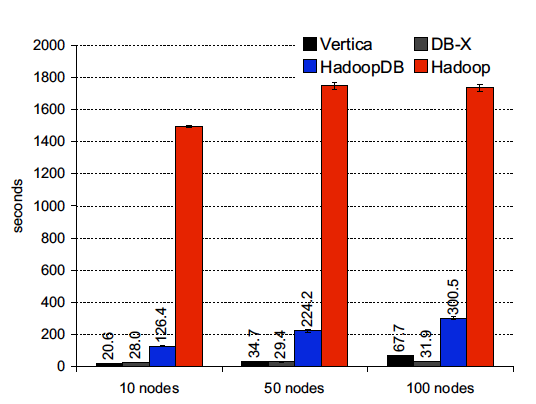
\includegraphics[width=0.5\textwidth]{Performance-Joint-Task}
    \end{center}
    \caption{\ttfamily{SELECT sourceIP, AVG(pageRank), SUM(adRevenue)
FROM rankings, uservisits
WHERE pageURL=destURL
AND visitDate BETWEEN 2000-1-15 AND 2000-1-22
GROUP BY sourceIP
ORDER BY SUM(adRevenue) DESC LIMIT 1;}}
 \end{figure}

% No full table scan due
% to clustered indexing
% 2 Hash partitioning and
% efficient join
% algorithm
% 3 Partial aggregation
% pushed into DB layer
\end{frame}

\begin{frame}
  \frametitle{Performance: Bottom Line}
  \begin{itemize}
  \item Unstructured data
    \begin{itemize}
    \item HadoopDB’s performance matches Hadoop
    \end{itemize}
  \end{itemize}
  
  \begin{itemize}
  \item Structured data
    \begin{itemize}
    \item HadoopDB’s performance is close to parallel databases
    \end{itemize}
  \end{itemize}
\end{frame}

\subsection{Scalability}

\begin{frame}
  \frametitle{Scalability: Setup}
  \begin{itemize}
  \item Simple aggregation task - full table scan
  \item Data replicated across 10 nodes
  \item Fault-tolerance: Kill a node halfway
  \item Fluctuation-tolerance: Slow down a node for the entire
    experiment
  \end{itemize}

  \begin{block}{Key differences}
    \begin{itemize}
    \item HadoopDB and Hadoop take advantage of runtime scheduling
      by splitting data into chunks or blocks
    \item Parallel databases restart wait for the slowest node
    \end{itemize}
  \end{block}
\end{frame}

\begin{frame}
  \frametitle{Scalability: Results}
  \begin{itemize}
  \item Run-time scheduling Block-level vs. Query-level restart
   \item Frequent checkpointing vs. pipelining results
  \end{itemize}
      \begin{center}
      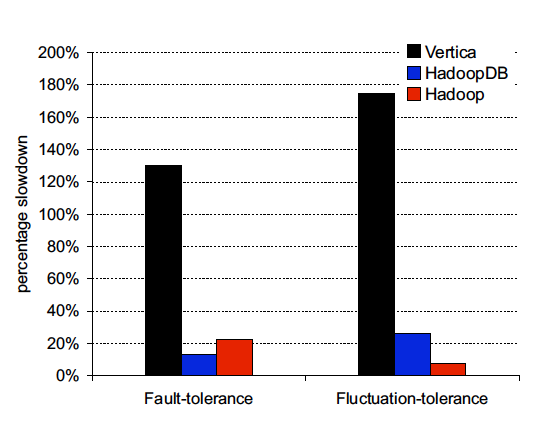
\includegraphics[width=0.6\textwidth]{Scalability-Result}
    \end{center}

\end{frame}

% \frame{

%   \frametitle{Our Ant Colony Based Approach on Longest Path}
%   \begin{block}{Input}
%     \begin{itemize}
%     \item Adjacency matrix representation of the input graph
%     \item Parameter for ACO: $\alpha$ and $\beta$
%     \end{itemize}
%   \end{block}

%   \begin{block}{Output}
%     \begin{itemize}
%     \item The \emph{Longest Path} (order of nodes to visit)
%     \item Cost of the \emph{Longest Path}
%     \end{itemize}
%   \end{block}

%   Most of the time $\alpha = 3$ and $\beta = 2$ produces the best
%   result [cite needed] }

% \subsection{The Heuristic Function}

% \frame{
%   \frametitle{The Heuristic Function}

%   \begin{block}{Value of the Heuristic Function $\eta(r, s)$}
%     \begin{itemize}
%     \item For weighted graphs, $\eta(r, s) = cost(r, s)$, where
%       $cost(r, s)$ is the weight/cost from node $r$ to node $s$
%     \item For un-weighted graphs, $\eta(r, s) = nbrcount(s)$ where
%       $nbrcount(s)$ is the number of neighbors of node $s$
%     \end{itemize}
%   \end{block}
% }

% \subsection{Local Search}

% \frame{
%   \frametitle{Local Search}
%   \begin{itemize}
%   \item It is a well known fact that basic ACO algorithm is prone to
%     \emph{Local optima}
%   \item Two types of \emph{Local Search} implemented to circumvent
%     this issue
%     \begin{itemize}
%     \item The Wise Ant
%     \item The Missing Vertex Checker
%     \end{itemize}
%   \item After all the ants have completed their tour, the local best
%     solution is put through these \emph{Local Search} procedures
%   \end{itemize}
% }

% \frame{\frametitle{Local Search: Procedure 1}
%   \begin{block}{Algorithm: The Wise Ant}
%     \begin{itemize}
%     \item Given a graph $G = (V, E)$ and a solution $S = [v_1, v_2,
%       v_3, \ldots ~ \ldots, v_m]$, pick two consecutive nodes $v_i,
%       v_{i+1}$ randomly from $S$ where $i \geq \lfloor m/2 \rfloor$
%     \item Reconstruct the solution with the added restriction that the
%       ant cannot go to $v_{i+1}$ from $v_i$
%     \end{itemize}
%   \end{block}
%   \begin{itemize}
%   \item If the local search produces a better solution, update the
%     local best solution with this one
%   \item To maximize efficiency, this search is applied to given
%     solution twice, in both forward and reverse order

%   \end{itemize}
% }

% \frame{
%   \frametitle{Example: The Wise Ant - Before Local Search}
%   Current cost is 43, current vertex is marked as \emph{grey}, tabu
%   vertex is marked as \emph{green}
%   \begin{center}
%     \includegraphics[width=0.7\textwidth]{lpath-before-wiseant}
%   \end{center}
% }

% \frame{
%   \frametitle{Example: The Wise Ant - After Local Search}
%   After local search cost is maximized to 45
%   \begin{center}
%     \includegraphics[width=0.7\textwidth]{lpath-best-sol}
%   \end{center}

% }

% \frame{
%   \frametitle{Local Search: Procedure 2}
%   Given a graph $G = (V, E)$, a solution $S = [v_1, v_2, v_3, \ldots ~
%   \ldots, v_m]$ and list of unvisited nodes $U = [u_1, u_2, u_3,
%   \ldots ~\ldots, u_{n-m}]$ % where $\forall{ v_i, u_j} \in V$,
%   do the following:
%   \begin{block}{Algorithm: The Missing Node Checker}
%     \begin{algorithmic}
%       \FORALL{$u_j \in U$} \FORALL{$v_i \in S$} \IF{$ cost(v_i, u_j) +
%         cost(u_j, v_{j+1}) \geq cost(v_i, v_{i+1})$} \STATE Insert
%       $u_j$ into $S$ after $v_i$
%       \ENDIF
%       \ENDFOR
%       \ENDFOR
%     \end{algorithmic}
%   \end{block}
% }

% \section{Experimental Results}
% \label{sec:experimental-results}

% \frame{\frametitle{Example: Missing Vertex Checker - Before Local
%     Search} Unvisited node is marked as \emph{green}, two of it's
%   adjacent visited nodes are marked as \emph{grey}, current cost is 38
%   \begin{center}
%     \includegraphics[width=0.7\textwidth]{lpath-missing-vertex-before}
%   \end{center}
% }

% \frame{\frametitle{Example: Missing Vertex Checker - After Local
%     Search} Missing vertex added to the path, now cost is 43
%   \begin{center}
%     \includegraphics[width=0.7\textwidth]{lpath-missing-vertex-after}
%   \end{center}
% }

% \frame{
%   \frametitle{Experimental Results}
%   \begin{itemize}
%   \item We compare our results with Portugal and Rocha's [cite needed]
%     \emph{Genetic Algorithm} (GA) based approach
%   \item They implemented 4 variants, two crossover based, one mutation
%     based and one variant have both mutation and crossover
%   \item Mutation based variant is the fastest one with good solution
%     quality, we compare ours results with this variant
%   \item We separately consider two type of graph classes,
%     \emph{sparse} and \emph{dense}
%   \end{itemize}
% }

% \subsection{Sparse Graphs}

% \frame{
%   \frametitle{Sparse Graphs}
%   \begin{itemize}
%   \item Input graph has 134 nodes and 134 edges with an optimum value
%     of 1556.0 for the longest path
%   \item The GA is run with 400 \emph{chromosomes} for 10 iterations
%   \item The ACO is run with 100 \emph{ants} for 10 iterations
%   \end{itemize}
%   \begin{block}{Comparison}
%     \begin{center}
%       \begin{tabular}[c]{c c c}
%         & Genetic Algorithm & ACO\\
%         \hline
%         Success Rate & 34.0\% & 90.0\%  \\
%         Quality &  95.7\% & 97.8\% \\
%         Avg. Running Time (ms) & 319.3 & 297.5 
%       \end{tabular}
%     \end{center}
%   \end{block}
%   Success rate is calculated by running the whole algorithm 100 times
% }

% \subsection{Dense Graphs}

% \frame{
%   \frametitle{Dense Graphs}
%   \begin{itemize}
%   \item Input graph has 30 nodes, 269 edges with optimum value 274.0
%     for longest path
%   \item The GA is run with 400 \emph{chromosomes} for 100 iterations
%   \item The ACO is run with 100 \emph{ants} for 100 iterations
%   \end{itemize}
%   \begin{block}{Comparison}
%     \begin{center}
%       \begin{tabular}[c]{c c c}
%         & Genetic Algorithm & ACO\\
%         \hline
%         Success Rate & 0\% & 20\%  \\
%         Quality &  89.6\% & 99.4\% \\
%         Avg. Running Time (ms) &  3546.7 & 2164.8 
%       \end{tabular}
%     \end{center}
%   \end{block}
% }

\section{Conclusion}
\label{sec:conclusion}

\subsection{Summary and Future Works}
\begin{frame}
  \frametitle{To Summarize}
  \begin{block}{HadoopDB ...}
    \begin{itemize}
    \item is a hybrid of DBMS and MapReduce
    \item scales better than commercial parallel databases
    \item is as fault-tolerant as Hadoop
    \item approaches the performance of parallel databases
    \item is free and open-source
    \end{itemize}
  \end{block}
\end{frame}

% \subsection{Future}

\begin{frame}
  \frametitle{Future Work}
  Engineering Work:
  \begin{itemize}
  \item Full SQL support in SMS 
  \item Data compression
  \item Integration with other open source databases
  \item Full automation of the loading and replication process
  \item Out-of-the box deployment
  \end{itemize}
  Research Work:
  \begin{itemize}
  \item Incremental loading and on-the-fly repartitioning
  \item Dynamically adjusting fault-tolerance levels based on failure
    rate
  \end{itemize}

\end{frame}


% \frame{
%   \frametitle{Conclusion}
%   \begin{itemize}
%   \item Preliminary results show that our ACO based implementation
%     performs way better than GA.
%   \end{itemize}
% }

\begin{frame}
  \frametitle{References}
  \begin{enumerate}
{\small{
  \item A. Abouzeid, K. Bajda-Pawlikowski, D. Abadi, A. Silberschatz, and A. Rasin. HadoopDB: An Architectural Hybrid of MapReduce and
    DBMS Technologies for Analytical Workloads. PVLDB, 2009.
  \item J. Dean and S. Ghemawat. MapReduce: Simplified Data Processing
    on Large Clusters. In OSDI, 2004.
  \item Michael Stonebraker, Daniel Abadi, David J. Dewitt, Sam Madden,
    Erik Paulson, Andrew Pavio, And Alexander Rasin, MapReduce and
    Parallel DBMSs -  Friends or Foes, Communications of ACM, 2011
    \item Kamil Bajda-Pawlikowski, Daniel J. Abadi, Avi Silberschatz,
      Erik Paulson. Efficient Processing of Data Warehousing Queries
      in a Split Execution Environment. VLDB, 2009
      \item Andrew Pavlo, 
Erik Paulson, Daniel J. Abadi, David J. DeWitt, Samuel Madden, Michael
Stonebraker. A Comparison of Approaches to Large-Scale Data
Analysis. CLUE 2010.}}
  \end{enumerate}
\end{frame}

\frame{
  \frametitle{Thank You}
  \begin{center}
    \LARGE{Questions \& Answers}
  \end{center}
}

\end{document}
